%%%%%%%%%%%%%%%%%%%%%%%%%%%%%%%%%%%%
% Slide options
%%%%%%%%%%%%%%%%%%%%%%%%%%%%%%%%%%%%

% Option 1: Slides with solutions

\documentclass[slidestop,compress,mathserif]{beamer}
\newcommand{\soln}[1]{\textit{#1}}
\newcommand{\solnGr}[1]{#1}

% Option 2: Handouts without solutions

%\documentclass[11pt,containsverbatim,handout]{beamer}
%\usepackage{pgfpages}
%\pgfpagesuselayout{4 on 1}[letterpaper,landscape,border shrink=5mm]
%\newcommand{\soln}[1]{ }
%\newcommand{\solnGr}{ }

%%%%%%%%%%%%%%%%%%%%%%%%%%%%%%%%%%%%
% Style
%%%%%%%%%%%%%%%%%%%%%%%%%%%%%%%%%%%%
\def\chp8@path{../../Chp 8}
\input{../../lec_style.tex}


%%%%%%%%%%%%%%%%%%%%%%%%%%%%%%%%%%%%
% Preamble
%%%%%%%%%%%%%%%%%%%%%%%%%%%%%%%%%%%%

\title[Lecture 33]{MA213: Lecture 33}
\subtitle{Module 5: Linear regression}
\author{OpenIntro Statistics, 4th Edition}
\institute{$\:$ \\ {\footnotesize Based on slides developed by Mine \c{C}etinkaya-Rundel of OpenIntro. \\
The slides may be copied, edited, and/or shared via the \webLink{http://creativecommons.org/licenses/by-sa/3.0/us/}{CC BY-SA license.} \\
Some images may be included under fair use guidelines (educational purposes).}}
\date{}


%%%%%%%%%%%%%%%%%%%%%%%%%%%%%%%%%%%%
% Begin document
%%%%%%%%%%%%%%%%%%%%%%%%%%%%%%%%%%%%

\begin{document}


%%%%%%%%%%%%%%%%%%%%%%%%%%%%%%%%%%%%
% Title page
%%%%%%%%%%%%%%%%%%%%%%%%%%%%%%%%%%%%

{
\addtocounter{framenumber}{-1} 
{\removepagenumbers 
\usebackgroundtemplate{\includegraphics[width=\paperwidth]{../../OpenIntro_Grid_4_3-01.jpg}}
\begin{frame}

\hfill \includegraphics[width=20mm]{../../oiLogo_highres}

\titlepage

\end{frame}
}
}


%%%%%%%%%%%%%%%%%%%%%%%%%%%%%%%%%%%%
% Recap/Agenda 
%%%%%%%%%%%%%%%%%%%%%%%%%%%%%%%%%%%%
% TODO better formatting
\begin{frame}
    \frametitle{Module 5: Linear regression}
    \begin{itemize}
        \item \hl{Previously: }Least squares regression (Chapter 8.2)
        \item \hl{This time: }Types of outliers in linear regression (Chapter 8.3)
        \item \hl{Reading: }Chapter 8.4 for next time
        \item \hl{Deadlines/Announcements: }HW 5.1 due Monday, Q4 in discussions next week
    \end{itemize}
    
\end{frame}
%%%%%%%%%%%%%%%%%%%%%%%%%%%%%%%%%%%%
% Sections
%%%%%%%%%%%%%%%%%%%%%%%%%%%%%%%%%%%%

%%%%%%%%%%%%%%%%%%%%%%%%%%%%%%%%%%%%

\section{Review}

\begin{frame}
    \frametitle{Last time: linear regression, $R^2$, extrapolation}
\end{frame}

\section{Types of outliers in linear regression}

%%%%%%%%%%%%%%%%%%%%%%%%%%%%%%%%%%%%

\begin{frame}
\frametitle{Types of outliers}

\twocol{0.5}{0.5}
{
\dq{How do outliers influence the least squares line in this plot?}

To answer this question think of where the regression line would be with and without the outlier(s). Without the outliers the regression line would be steeper, and lie closer to the larger group of observations. With the outliers the line is pulled up and away from some of the observations in the larger group. 
}
{
\begin{center}
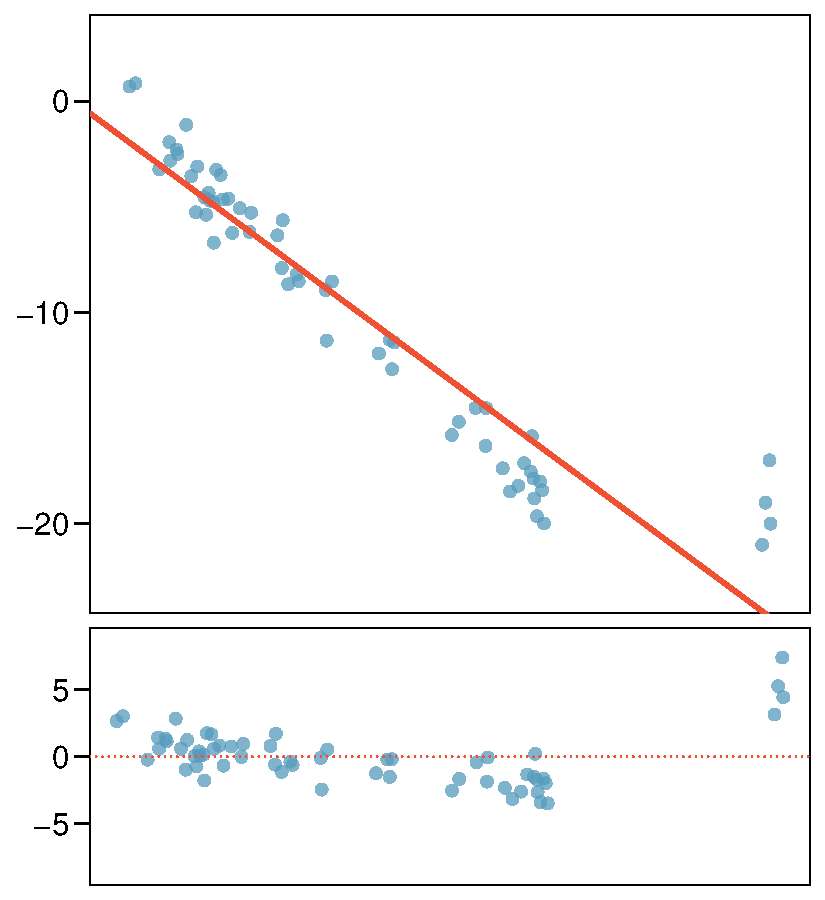
\includegraphics[width=\textwidth]{\chp8@path/8-3_outliers/figures/outlierPlots/out4}
\end{center}
}

\end{frame}

%%%%%%%%%%%%%%%%%%%%%%%%%%%%%%%%%%%

\begin{frame}
\frametitle{Types of outliers}

\twocol{0.4}{0.6}
{
\dq{How do outliers influence the least squares line in this plot?} \\
\soln{\only<2>{Without the outlier there is no evident relationship between $x$ and $y$.}}
}
{
\begin{center}
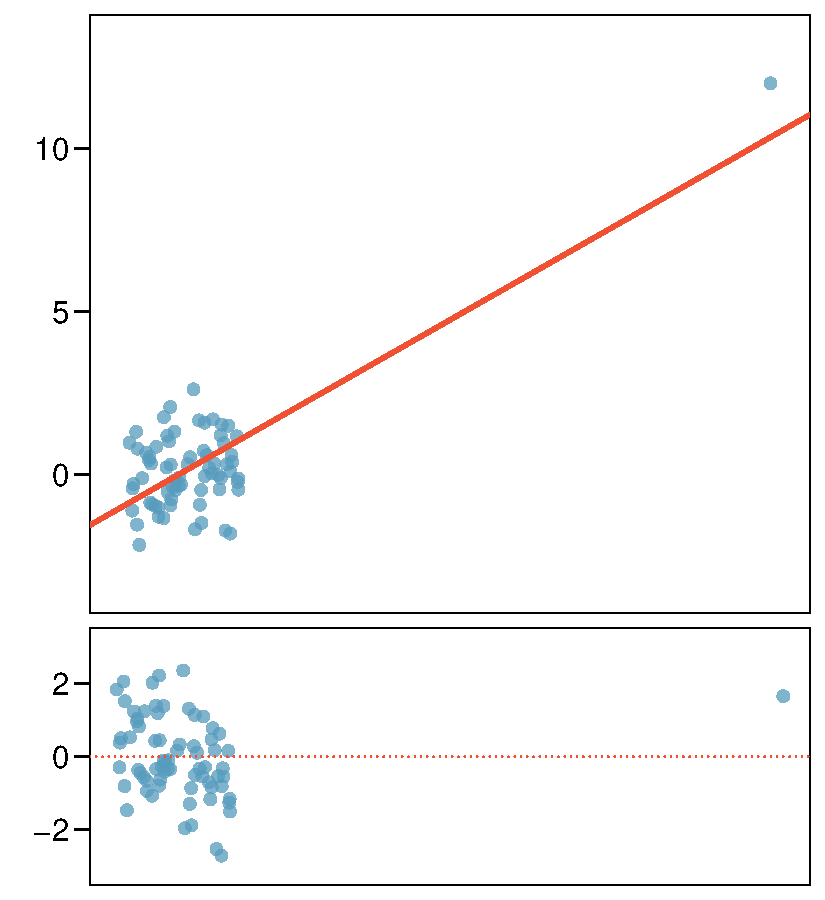
\includegraphics[width=\textwidth]{\chp8@path/8-3_outliers/figures/outlierPlots/out5}
\end{center}
}

\end{frame}

%%%%%%%%%%%%%%%%%%%%%%%%%%%%%%%%%%%

\begin{frame}
\frametitle{Some terminology}
 
\begin{itemize}

\item \hl{Outliers} are points that lie away from the cloud  of points.

\pause

\item Outliers that lie horizontally away from the center of the cloud are called \hl{high leverage} points.

\pause

\item High leverage points that actually influence the \underline{slope} of the regression line are called \hl{influential} points.

\pause

\item In order to determine if a point is influential, visualize the regression line with and without the point. Does the slope of the line change considerably? If so, then the point is influential. If not, then it?s not an influential point.

\end{itemize}

\end{frame}

%%%%%%%%%%%%%%%%%%%%%%%%%%%%%%%%%%%

\begin{frame}
\frametitle{Influential points}

Data are available on the log of the surface temperature and the log of the light intensity of 47 stars in the star cluster CYG OB1.

\twocol{0.7}{0.3}
{
\begin{center}
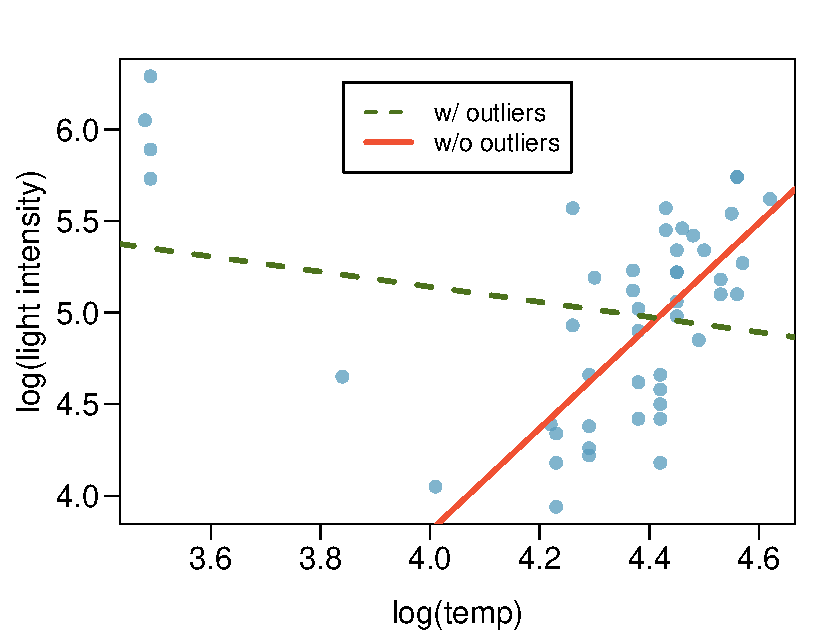
\includegraphics[width=\textwidth]{\chp8@path/8-3_outliers/figures/stars/star}
\end{center}
}
{
\begin{center}
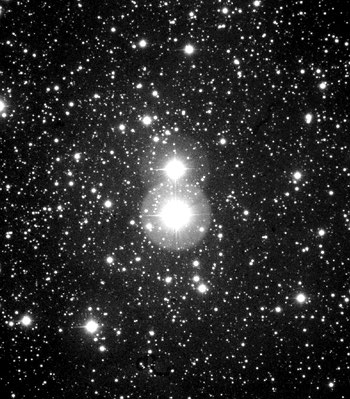
\includegraphics[width=\textwidth]{\chp8@path/8-3_outliers/figures/stars/cyg}
\end{center}
}

\end{frame}

%%%%%%%%%%%%%%%%%%%%%%%%%%%%%%%%%%%

\begin{frame}
\frametitle{Types of outliers}

\twocol{0.4}{0.6}
{
\pq{Which of the below best describes the outlier?}
\begin{enumerate}[(a)]
\item influential
\solnMult{high leverage}
\item none of the above
\item there are no outliers
\end{enumerate}
}
{
\begin{center}
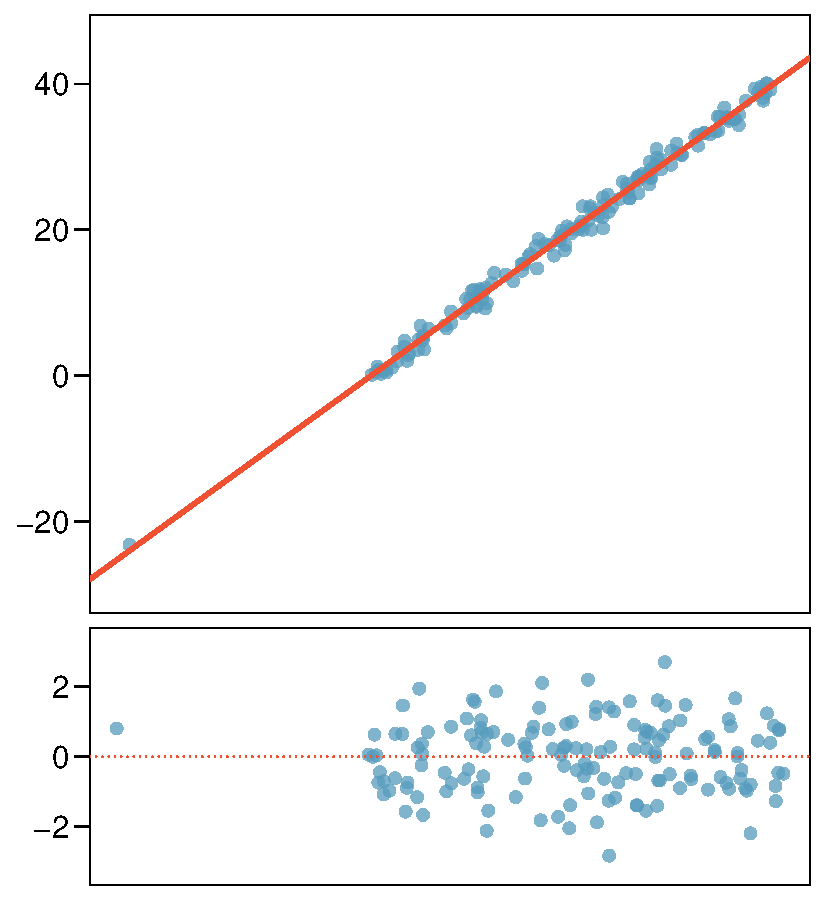
\includegraphics[width=\textwidth]{\chp8@path/8-3_outliers/figures/outlierPlots/out6}
\end{center}
}

\end{frame}

%%%%%%%%%%%%%%%%%%%%%%%%%%%%%%%%%%%

\begin{frame}
\frametitle{Types of outliers}

\twocol{0.4}{0.6}
{
\dq{Does this outlier influence the slope of the regression line?}
\soln{\only<2>{Not much...}}

}
{
\begin{center}
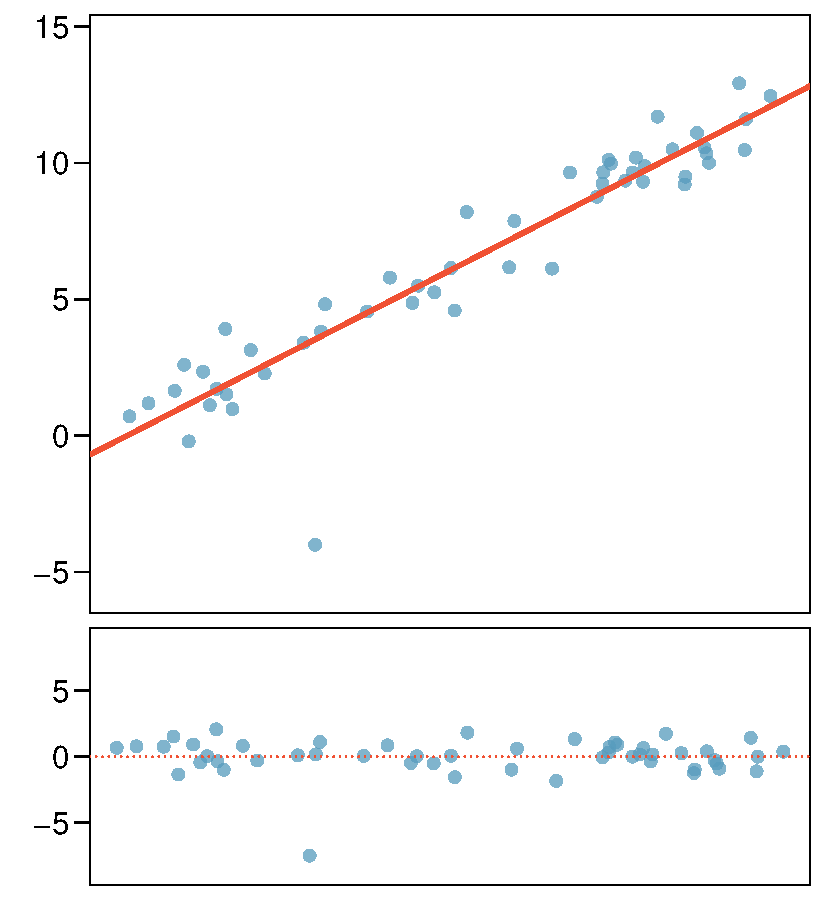
\includegraphics[width=\textwidth]{\chp8@path/8-3_outliers/figures/outlierPlots/out1}
\end{center}
}

\end{frame}

%%%%%%%%%%%%%%%%%%%%%%%%%%%%%%%%%%%

\section{R Demonstration: Influential points and the best-fit line}

%%%%%%%%%%%%%%%%%%%%%%%%%%%%%%%%%%%

\begin{frame}
\frametitle{Recap}

\pq{Which of following is \underline{true}?}

\begin{enumerate}[(a)]
\item Influential points always change the intercept of the regression line.
\item Influential points always reduce $R^2$.
\item It is much more likely for a low leverage point to be influential, than a high leverage point.
\item When the data set includes an influential point, the relationship between the explanatory variable and the response variable is always nonlinear.
\solnMult{None of the above.}
\end{enumerate}

\end{frame}

%%%%%%%%%%%%%%%%%%%%%%%%%%%%%%%%%%%

\begin{frame}
\frametitle{Recap (cont.)}

\vspace{-1cm}

\twocol{0.5}{0.5}
{
\begin{center}
\[ R = 0.08, R^2 = 0.0064 \]
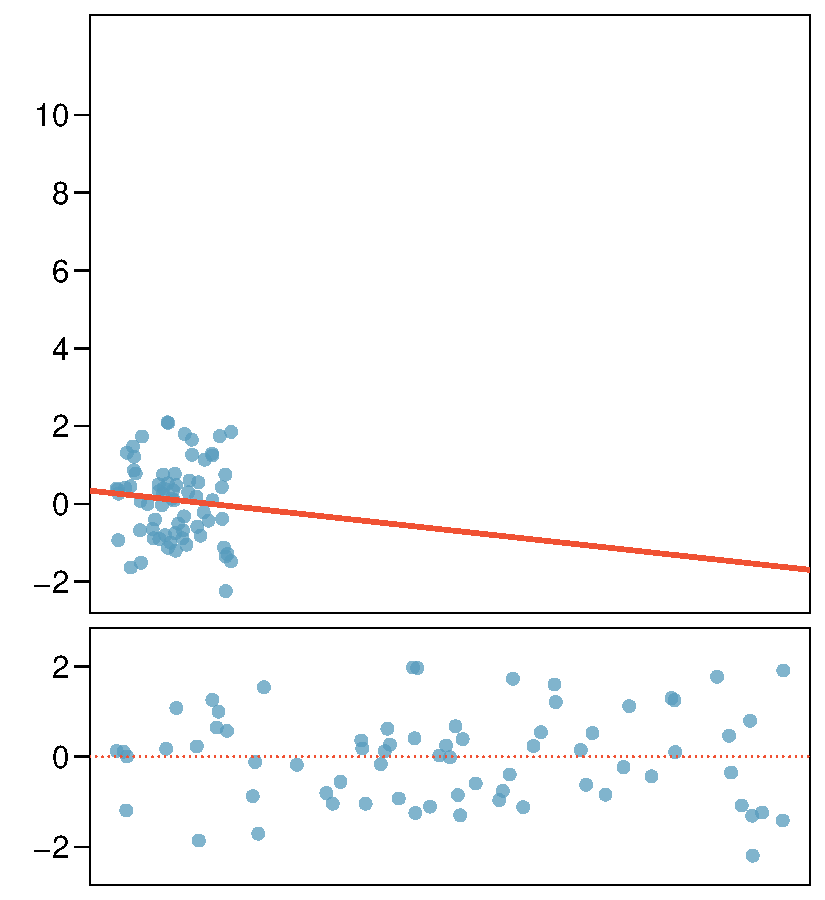
\includegraphics[width=\textwidth]{\chp8@path/8-3_outliers/figures/outlierPlots/out5-1}
\end{center}
}
{
\begin{center}
\[ R = 0.79, R^2 = 0.6241 \]
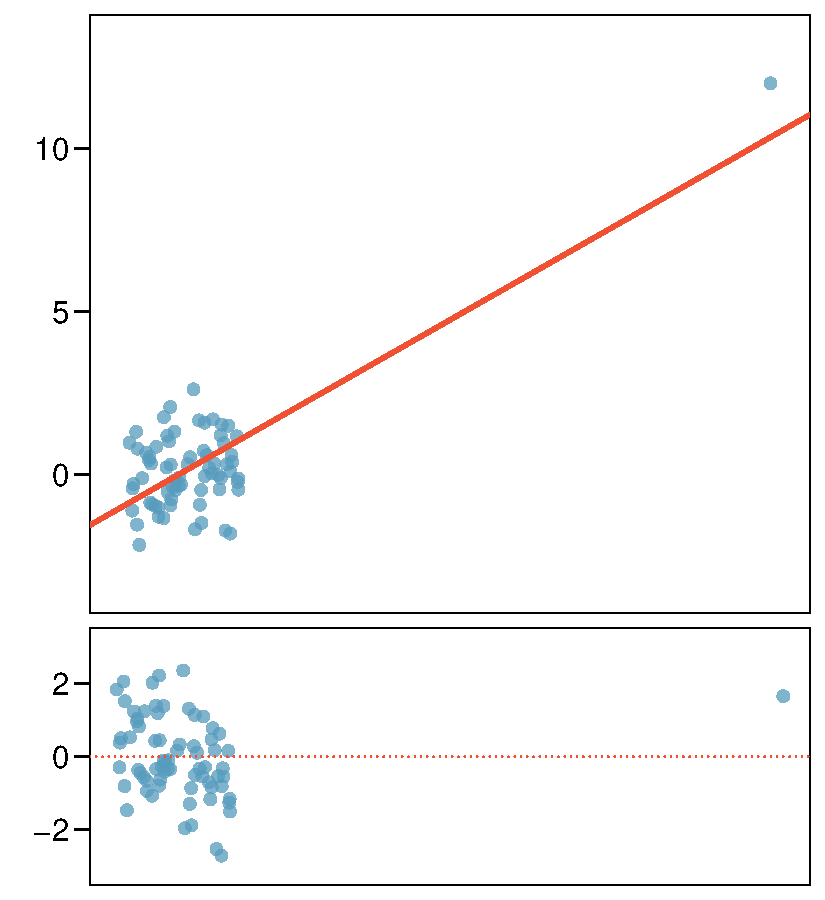
\includegraphics[width=\textwidth]{\chp8@path/8-3_outliers/figures/outlierPlots/out5}
\end{center}
}

\end{frame}

%%%%%%%%%%%%%%%%%%%%%%%%%%%%%%%%%%%%
% End document
%%%%%%%%%%%%%%%%%%%%%%%%%%%%%%%%%%%%

\end{document}
